\chapter{A Hyperplane-based Data Reconstruction Attack in Federated Learning}\label{chap:ctp}

This chapter is based on our paper \citeA{ctp_paper}, published at the Forty-First Conference on Uncertainty in Artificial Intelligence (UAI 2025).
 
\paragraph{Chapter Summary} Analytical data reconstruction attacks in federated learning can exactly recover private inputs from model gradients, but their effectiveness deteriorates substantially as the batch size increases and, in many cases, depends on prior knowledge of the clients' data distribution or access to auxiliary data. In this chapter, we first provide a geometric interpretation of sparsity-based reconstruction attacks and show that their ability to isolate individual samples is fundamentally constrained by the dimensionality of the input space. We then introduce a hyperplane-based reconstruction attack for the malicious-server setting that overcomes these limitations. Our approach exploits the activation boundaries of fully connected ReLU layers to partition the input space with parallel hyperplanes and progressively isolate individual records. By controlling the contribution of each sample to the observed gradients and adaptively refining the resulting partition across communication rounds, the adversary can analytically reconstruct the entire client batch without prior knowledge of its data distribution or access to auxiliary data. The search is parallelized across the neurons of the attacked layer, allowing a large number of candidate hyperplanes to be evaluated within each communication round. Experiments on both image and tabular classification tasks demonstrate that the proposed attack substantially outperforms existing analytical methods and achieves perfect reconstruction of batches containing up to 4096 samples, two orders of magnitude larger than those recovered by the considered state-of-the-art baseline. These results show that large-batch aggregation and low input dimensionality alone do not provide effective protection against a malicious federated learning server.

\section{Motivation}

In Section~\ref{sec:dra}, we discussed how federated learning is vulnerable to data reconstruction attacks (DRAs), often referred to as gradient inversion attacks (GIAs), in which an adversary attempts to recover the private training records of a client from the information exchanged during training. Despite substantial progress in this area, existing attacks present important limitations. Optimization-based methods generally struggle as the number of samples contributing to an update increases, while several malicious-server attacks rely on auxiliary data or prior knowledge of the clients' data distribution. Analytical attacks can instead provide exact reconstruction, but existing approaches are difficult to scale to large batches and are particularly ineffective on low-dimensional data. Consequently, no existing approach simultaneously provides exact reconstruction, scales to large batches, and remains effective on low-dimensional tabular data without relying on strong auxiliary assumptions.

This last limitation is particularly relevant because most reconstruction attacks have been developed and evaluated primarily on image data, whereas many privacy-sensitive applications, including clinical and financial applications, rely on tabular records. 

Motivated by these observations, in this chapter we consider a \emph{malicious-server} setting, in which the server can modify the model parameters sent to a targeted client in order to amplify privacy leakage. We first provide a geometric interpretation of existing sparsity-based analytical attacks and show that their ability to isolate individual records is fundamentally constrained by the dimensionality of the input space. We then introduce a different reconstruction strategy that combines a geometric search in the feature space with precise control over each sample's contribution to the client's gradients. The central idea is to progressively isolate individual records within strips delimited by parallel hyperplanes and reconstruct them from the changes observed as these hyperplanes move across the input space. By parallelizing this search across the neurons of a fully connected layer and refining it over multiple communication rounds, the attacker can progressively recover the complete client batch without requiring auxiliary data or prior knowledge of its distribution.

Concretely, the main contributions of this chapter are the following:
\begin{itemize}
    \item We provide a geometric interpretation of existing sparsity-based analytical attacks and derive an analytical upper bound on their reconstruction capabilities for random data.

    \item We show how a malicious server can manipulate the model parameters to control each data point's contribution to the gradients observed during federated training.

    \item We introduce a hyperplane-based reconstruction algorithm for classification tasks that is agnostic to the input dimensionality. Given sufficiently many communication rounds, the proposed method can recover the complete client batch independently of its size and can therefore be applied to both image and tabular data. \francesco{The attack in practice works also for regression, but this is something that we evaluated in the VGIA paper, and at the time, did not test here. So, I am not sure if to keep the discussion classification-oriented, as in the original paper, or to extend also to regression}

    \item We validate the proposed attack on image and tabular datasets, demonstrating perfect reconstruction of batches containing up to $4{,}096$ samples, while the considered state-of-the-art baseline fails to perfectly recover batches of only $64$ samples. 
    \francesco{Double check Robbing the Fed performance. On this last point I might be more careful.}
\end{itemize}

\section{Problem Description and Background}\label{sec:ctp_background}

We consider the federated learning setting introduced in Section~\ref{sec:fed_learning}, with global objective given in Equation~\ref{eq:globalobjective}. In this setting, the server observes updates computed from clients' local data, where the contributions of multiple training samples are typically aggregated together. As discussed in Section~\ref{sec:dra}, disentangling these contributions represents a major obstacle for data reconstruction attacks. In the honest-but-curious setting, the adversary has no control over how individual samples contribute to the observed update, and existing attacks generally become ineffective as the batch size increases. Optimization-based attacks face an additional limitation: reconstruction is obtained by solving a non-convex gradient-matching problem and is therefore not guaranteed to recover the original inputs exactly, often producing noisy or erroneous samples even when the attack succeeds. A malicious server can alleviate the aggregation problem by manipulating the model sent to the client to amplify or isolate individual gradient contributions. Existing optimization-based attacks in this setting, however, often rely on additional information, such as prior knowledge of the distribution of an input feature~\cite{wenFishingUserData2022a} or access to auxiliary data~\cite{garovHidingPlainSight2024}. These limitations motivate the analytical approach adopted in this chapter.

The limitations of optimization-based reconstruction motivate the analytical approach~\cite{phong_gia,fowlRobbingFedDirectly2021} considered in this chapter. Analytical attacks exploit algebraic relationships between the gradients of fully connected layers and the samples that generated them, allowing exact input recovery when suitable activation patterns are obtained. The main challenge consequently shifts from solving an approximate reconstruction problem to obtaining gradient observations that isolate the contribution of a single sample from the remaining records in the batch.


To formalize this idea, consider a client training a neural network containing a fully connected (FC) layer followed by a ReLU activation. Let $\x \in \mathbb{R}^{d}$ and $\z \in \mathbb{R}^{N}$ denote, respectively, the input to the layer and its output after the ReLU activation. In particular, when the considered layer is the input layer of the network, $\x$ coincides with the original data sample.
Let $\W \in \mathbb{R}^{N \times d}$ and $\b \in \mathbb{R}^{N}$ denote the weight matrix and the bias vector, respectively. 
The output of the $i$-th neuron in the layer is $z_i = \relu(\W_i \x + b_i)$. 
Given a sample $(\x_j, y_j)$, let $\loss_j$ and $z_{i,j}$ denote the loss and the output of neuron~$i$ for this sample, respectively. The gradient of the loss with respect to $\W_i$ and $b_i$ can be computed as follows\footnote{
 The expression $\frac{\partial\mathbf{f}}{\partial \x}$, where $\mathbf{f}: \mathbb R^d \to \mathbb{R}^N$, can also be interpreted as the Jacobian of the function $\mathbf f$, with the (less common) convention that 
$\left(\frac{\partial\mathbf{f}}{\partial \x}\right)_{i,j} = \frac{\partial f_j}{\partial x_i}$.
}:
\[
\frac{\partial \loss_j}{\partial \W_i}
=
\frac{\partial \loss_j}{\partial z_i}
\frac{\partial z_i}{\partial \W_i}
=
\frac{\partial \loss_j}{\partial z_i}
\x_j
\indicator{z_{i,j}>0},
\]

while the gradient with respect to $b_i$ is

\[
\frac{\partial \loss_j}{\partial b_i}
=
\frac{\partial \loss_j}{\partial z_i}
\frac{\partial z_i}{\partial b_i}
=
\frac{\partial \loss_j}{\partial z_i}
\indicator_{z_{i,j}>0}.
\]

It follows that

\[
\frac{\partial \loss_j}{\partial \W_i}
=
\frac{\partial \loss_j}{\partial b_i}
\x_j.
\]

Consequently, as long as

\[
\frac{\partial \loss_j}{\partial b_i} \neq 0,
\]

which requires that $\x_j$ activates neuron $i$, namely

\[
\W_i \x_j + b_i > 0,
\]

knowing the gradient of the model loss enables exact reconstruction of the input:

\begin{equation}\label{eq:single_input_rec}
\x_j
=
\frac{\partial \loss_j}{\partial \W_i}
\left(
\frac{\partial \loss_j}{\partial b_i}
\right)^{-1}.
\end{equation}



However, in practice, gradients are computed on a batch $\batch=\{(\x_j, y_j)\}_{j=1}^n$ of size $n$, rather than on a single input. %Let $\loss_j$ denote the loss of the model on sample $(\x_j, y_j)$. 
The attacker can then only observe the  gradient of the average loss $\loss = \frac{1}{n} \sum_{j=1}^n \loss_j$:
\begin{equation}\label{eq:aggr_obs}
     \frac{\partial \loss}{\partial \W_i} =  \frac{1}{n} \sum_{j=1}^n \frac{\partial \loss_j}{\partial b_i}\x_j \, \\
\end{equation}
\begin{equation}\label{eq:aggr_coeff}
     \frac{\partial \loss}{\partial b_i} =  \frac{1}{n} \sum_{j=1 }^n \frac{\partial \loss_j}{\partial b_i}.\\
\end{equation}
If $\frac{\partial \loss}{\partial b_i}\neq 0$---implying that at least one input activates neuron~$i$---the attacker can reconstruct a combination $\o_i$ of the inputs from this gradient \cite[Theorem~1]{ZHANG2023119421}:
%(i.e., at least one input activates neuron $i$), 

\begin{align}
    \o_i &= \frac{\partial{\loss}}{\partial{\W_i}} \cdot \left( \frac{\partial{\mathcal{L}}}{\partial{b_i}} \right) ^{-1} = \sum_{j=1}^n \alpha_j \x_j, \label{eq:obs_derivation} \\
    \alpha_j &=  \frac{\frac{\partial{\loss_j}}{\partial{b_{i}}}} {\sum^{n}_{k=1} \frac{\partial{\loss_k}}{\partial{b_{i}}}}.\label{eq:alpha_derivation}
\end{align}
Equations~\ref{eq:obs_derivation}  and \ref{eq:alpha_derivation} are the starting points for different attacks.


As discussed in Section~\ref{sec:dra}, several analytical attacks exploit the sparsity induced by activation functions to separate individual samples from aggregated gradients. In the following, we focus on malicious sparsity-based attacks such as those proposed by~\citeA{boenischWhenCuriousAbandon2023} and~\citeA{ZHANG2023119421}. These attacks manipulate the parameters of a fully connected layer to increase the number of neurons that are activated by a single input in the client batch. Whenever such an activation pattern is obtained, the contribution of that neuron corresponds to a single sample, which can be reconstructed exactly through~\eqref{eq:single_input_rec}.

Their effectiveness therefore depends on how many samples in the batch can be isolated from all the others through the activation region of a neuron. In the next section, we characterize this condition geometrically and show that it imposes a fundamental limitation on the reconstruction capabilities of this class of attacks.

Other analytical attacks rely instead on differences between activation sets to isolate individual samples. For instance, \citeA{fowlRobbingFedDirectly2021} configure neurons with different activation thresholds so that the difference between their gradients reveals the contribution of a single input. Related constructions have subsequently extended this principle to other settings, including secure aggregation~\cite{zhaoLOKILargescaleData2023a}, Transformer models~\cite{fowlDecepticonsCorruptedTransformers2022,chu2023panning}, and the reconstruction from intermediate representations~\cite{shiScaleMIAScalableModel2025}. However, these approaches rely on additional prior information related to the victim's data distribution, such as knowledge of the distribution of a projection of the inputs~\cite{fowlRobbingFedDirectly2021,fowlDecepticonsCorruptedTransformers2022,chu2023panning, zhaoLOKILargescaleData2023a} or access to auxiliary data drawn from a similar distribution~\cite{shiScaleMIAScalableModel2025}.

\section{Limitations of Existing Sparsity-Based Attacks}\label{sec:limit}

The sparsity-based attacks proposed by \citeA{boenischWhenCuriousAbandon2023, ZHANG2023119421} attempt to modify the parameters of the first FC layer so that each neuron in the layer is activated only by a single input.
Given the batch  $\mathcal{B}=\{(\x_1, y_1) \dots, (\x_n, y_n)\}$, neuron $i$ is activated only from input $\x_j$ if $\W_i \x_j+b_i>0$ and $\W_i \x_k+b_i<0$ for $k \in \{1, \dots, n\}\setminus \{j\}$.
In this section we provide a geometric interpretation of the problem and demonstrate that the accuracy of sparsity-based attacks is fundamentally constrained by the dimensionality of the input they aim to reconstruct.

Consider the set of inputs for which the activation value of neuron $i$ is equal to $0$, i.e., $    \{ \x \in \mathbb{R}^d \mid \W_i\x + b_i= 0\}$.
This set is a hyperplane in the Euclidean space $\mathbb R^d$ orthogonal to the vector $\W_i$.

The attacks proposed by \citeA{boenischWhenCuriousAbandon2023, ZHANG2023119421} can be interpreted as identifying hyperplanes orthogonal to random directions $\W_i$ that separate a single input from the rest of the inputs in the batch, which we denote by $\batch_{\x}= \{\x_1, \x_2, \dots, \x_n\}$. Given a gradient computed on the batch $\batch$, the maximum number of recoverable points is upper-bounded by the number of points in $\batch_{\x}$ that are linearly separable from all the others, i.e., the number of vertices on the convex hull of $\batch_{\x}$. By bounding the expected number of vertices, we derive the following theorem:

\begin{theorem}
\label{theo:active_bound}
Let the input features of the client's local dataset consist of $n$ random points in $\mathbb{R}^d$ that are drawn
\begin{enumerate}
    \item uniformly at random from the unit ball, or
    \item uniformly at random from the unit hypercube, or
    \item from a centered normal distribution with covariance matrix $\mathbf{I}_d$.
\end{enumerate}
Consider training a machine learning model through FedSGD with full-batch updates. The expected number of samples that can be reconstructed by any attack relying on isolating individual inputs from the rest of the batch is:
\begin{enumerate}
    \item $O(n^{(d-1)/(d+1)})$, %or
    \item $O(\log^{d-1} n)$, %or
    \item $O(\log^{(d-1)/2} n)$,
\end{enumerate}
respectively for the three distributions above.
\end{theorem}

Theorem~\ref{theo:active_bound} shows that, for a fixed input dimension $d$, the expected fraction of reconstructed samples---i.e., the attack success rate---approaches zero asymptotically as the batch size $n$ increases. This result explains the attack performance degradation observed by \cite{boenischWhenCuriousAbandon2023, ZHANG2023119421} when larger batch sizes are used.
Furthermore, the theorem highlights a fundamental limitation in low-dimensional settings: the smaller the input dimension~$d$, the lower the success rate. 
This indicates that while such attacks can succeed in high-dimensional regimes, their effectiveness diminishes substantially when applied to low-dimensional data. Moreover, high-dimensional data often lies on manifolds of much lower intrinsic dimensionality~\cite{NIPS2010_8a1e808b, pope2021the, brown2023verifying}, potentially reducing the success rate of these attacks even further than predicted by Theorem~\ref{theo:active_bound}.

\section{The Cutting Through Privacy Attack} \label{sec:our_attack}
In this Section, we first present our threat model (Section~\ref{sec:threat}) and then introduce our attack assuming the attacker initially exploits a single neuron in the linear layer (Section~\ref{sec:loc_and_rec} and~\ref{sec:control_weights}). We subsequently demonstrate how the attacker can leverage all neurons in parallel to significantly accelerate the reconstruction process (Section~\ref{sec:parallel}).

\subsection{Threat Model}\
\label{sec:threat}
In this chapter, we consider a malicious server whose intent is to recover clients' private data by altering model parameters, consistent with the setting presented in Section~\ref{subsec:threatmodel} and described in \cite{wenFishingUserData2022a, boenischWhenCuriousAbandon2023, ZHANG2023119421}, where clients trust the server and have no control over the model parameters.
We note that a third party capable of intercepting communications between the client and server could also act as an attacker.

Additionally, since the central server orchestrates the FL protocol, we assume that it is responsible for selecting the clients participating in each training round. 
Unlike previous works \cite{fowlRobbingFedDirectly2021, wenFishingUserData2022a,boenischWhenCuriousAbandon2023,ZHANG2023119421,zhaoLOKILargescaleData2023a}, we assume the server has no knowledge of the clients' data distribution and does not possess any auxiliary training data. The information available to the server is limited to some bounds on the range of the data after preprocessing.
We suppose that clients follow the FedSGD protocol and at each round compute a full-batch gradient update. 
\subsection{Locate and Reconstruct the Inputs}\label{sec:loc_and_rec}
Consider that the client under attack has dataset $\localdataset$ with corresponding inputs $\batch_{\x}$.

For simplicity, we assume that the neural network consists solely of a FC input layer with ReLU activations (with parameters $\Win \in \mathbb{R}^{N \times d}$ and $\bin \in \mathbb{R}^{N}$) and a FC classification layer (with parameters $\W^{L} \in \mathbb{R}^{C\times N}$ and $\b^{L} \in \mathbb{R}^{C}$). The output of the network can be expressed as $\z^{L}=\W^{L}\z^{a}+\b^{L} \in \mathbb{R}^C$, where $\z^{a}~=\relu(\W^{a}\x+\b^{a}) \in \mathbb{R}^N$.
The attack can also be extended to fully connected networks with an arbitrary number of layers $L>2$, as well as to other architectures by incorporating model modifications proposed in previous works. In Section~\ref{sec:ctp_experiments}, for example, we evaluate the attack on convolutional neural networks by adapting the modifications introduced by~\citeA{boenischWhenCuriousAbandon2023}. An analogous extension to Transformer architectures can be obtained by modifying the attention layers following the construction proposed by~\citeA{fowlDecepticonsCorruptedTransformers2022}. 
The server selects a random hyperplane by sampling $\Win_i$ from an arbitrary random distribution. During different communication rounds, it sends the client under attack a model whose parameters are constant except for the bias value $\bini$.
Geometrically, changing $\bini$ corresponds to translating the hyperplane through the input space (see Figure~\ref{fig:geometry}). The goal is to find a sequence of scalars $\hat b^{a}_{i,0} \leq \dots \leq \hat b^{a}_{i,n}$ such that for each consecutive pair of hyperplanes $\Win_i \x + \hat b^{a}_{i,k} = 0$ and $\Win_i \x + \hat b^{a}_{i,k+1} = 0$, exactly one input $\x_j$ in the client's local dataset lies in-between them.
%, that is $\Win_i \x_j + b^{a}_{i,k} < 0$ 
Note that as the bias transitions between consecutive values in the sequence, a single additional input activates the neuron $i$.

We now explain how the server determines this sequence of bias values and how it can reconstruct the isolated samples. To facilitate the exposition, we introduce an assumption here, which we justify in Sec.~\ref{sec:control_weights}.

\begin{assumption}\label{ass:grad}
%For every input $\x_j \in \localdataset_{\x}$ and the values of $b^{a}_i$ tested by the attacker, if neuron $i$ is activated by input $\x_j$ for the specific value of $b^{a}_i$, the derivative $\frac{\partial \loss_j}{\partial z^{a}_i}$ does not depend on $b_i^{a}$.
For each input $(\x_j, y_j) \in \localdataset$ and each value of $b^{a}_i$
%values $b^{a}_i$ 
tested by the attacker, if neuron $i$ is activated by the input $\x_j$ for a given value of $b^{a}_i$, the derivative ${\partial \loss_j}/{\partial b^{a}_i}$ remains independent of $b^{a}_i$. %\textcolor{blue}{SUGGEST TO REMOVE: and $\alpha_{j}$~\eqref{eq:alpha_derivation} is non-negligible.}
% If an input $\x_j$ activates the $i$-th neuron, the gradient of its loss with respect to $\z^{a}_i$ remains constant across different communication rounds, i.e., $\forall \x_j \in \batch_{\x}$:
% \begin{equation*}
%     \frac{\partial \loss_j}{\partial z_i}(t)=\frac{\partial \loss_j}{\partial z_i}(t+1)
% \end{equation*}
% where $t \in \{1,\dots T\}$ indicates the communication round.
\end{assumption}

According to \eqref{eq:obs_derivation}, for a given bias value $b^{a}_{i,k}$, the server observes the client's aggregate gradient $\o_k = \sum_{j=1}^n \alpha_{j,k} \x_j$. Given hyperplanes $\Win_i \x + b^{a}_{i,k} = 0$ and $\Win_i \x + b^{a}_{i,k+1} = 0$, the attacker can determine whether they enclose at least one point by comparing $\o_{k}$ and $\o_{k+1}$. Indeed, if there is no input point between the two hyperplanes, the same set of inputs activates neuron~$i$ and $\alpha_{i,k} = \alpha_{i,k+1}$ (because of Assumption~\ref{ass:grad}), then $\o_k=\o_{k+1}$. If $\o_k\neq\o_{k+1}$, then the server knows that there is at least one input in-between and, by binary search, can progressively isolate the inputs as far as their projections along the direction $(\W_i^{a})^\intercal$ differ by more than a threshold~$\varepsilon$ (see Appendix~\ref{app:bound_on_rounds} for its configuration rule).

After isolating all the input points, the attacker can reconstruct the inputs sequentially from $\x_1$ to $\x_n$, where we relabel the inputs so that $\x_j \in \batch_{\x}$ is the input between the two hyperplanes corresponding to $\hat b^{a}_{i,j-1}$ and $\hat b^{a}_{i,j}$. 
Input $\x_1$ can be directly reconstructed using \eqref{eq:single_input_rec} with the client's loss gradient computed for $\hat b^{a}_{i,1}$. We note that the attacker also knows ${\partial \loss_1}/{\partial b^{a}_i}$ for $b^{a}=\hat b^{a}_{i,1} $, i.e., when $\x_1$ activates neuron~$i$. Suppose now that the attacker already reconstructed the first $k$ inputs $\x_1, \dots, \x_k$ and the corresponding partial derivatives ${\partial \loss_1}/{\partial b^{a}_i}, \dots, {\partial \loss_k}/{\partial b^{a}_i}$ when the corresponding inputs activate neuron $i$.
Let $h_k$ denote the partial derivative of the loss for $\hat{b}^{a}_{i,k}$, i.e., $h_k ={\partial \loss }/{\partial b^{a}_{i}}$.
Due to \eqref{eq:aggr_coeff} and Ass.~\ref{ass:grad}, the attacker can reconstruct ${\partial \loss_{k+1}}/{\partial b^{a}_i}$ by
\begin{equation}
\frac{\partial \loss_{k+1}}{\partial b^{a}_i}= n (h_{k+1} - h_k).
\end{equation}
The attacker can then compute the set of coefficients $\alpha_{j,k+1}$ in the linear combination of $\o_{k+1}$ in \eqref{eq:alpha_derivation} and reconstruct $\x_{k+1}$ by
\begin{equation}\label{eq:input_rec}
\x_{k+1} = \frac{\o_{{k}+1} - \sum_{j=1}^{k} \alpha_{j,k+1} \x_j}{\alpha_{j,k+1}}.
\end{equation}
\francesco{this has to be corrected and stated more carefully. In practice we do not require to do the two things consecutively, but they can be interleaved and moreover, a wrong reconsrtuction does not imply that the method breaks}

While we have described the process in two consecutive phases---first isolating the inputs with the hyperplanes and then reconstructing the inputs---we note that these procedures can be intertwined. In particular, inputs $\x_1, \dots, \x_k$ can be reconstructed as soon as the corresponding bias values $\hat b^{a}_{i,1}, \dots, \hat b^{a}_{i,k}$ have been identified.

\begin{figure}[t]
    \centering
    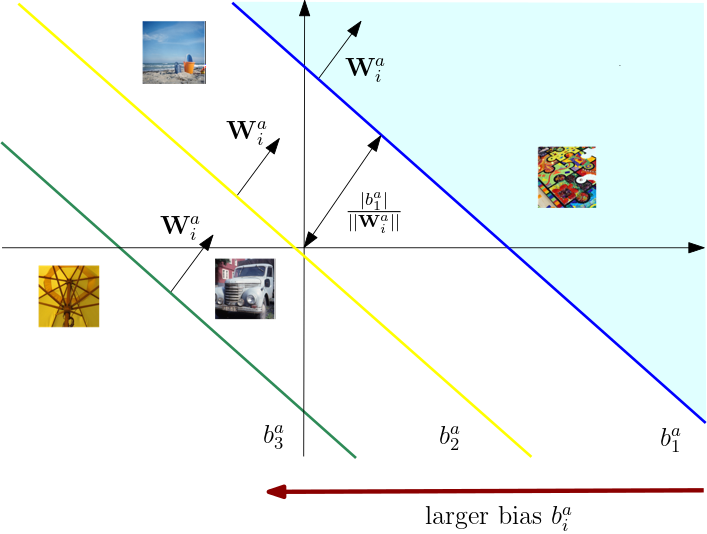
\includegraphics[width=0.6\linewidth]{assets/chapter_3/hp_example.png}
    \caption{Illustration of our attack strategy, in which hyperplanes are positioned to isolate a single image within the strip they define. The light-blue region represents  the half-space where $\Win_i \x + b_1^{a} > 0$.}
    \label{fig:geometry}
\end{figure}
\subsection{Controlling the Gradients}\label{sec:control_weights}

Assumption~\ref{ass:grad} requires  that the gradients ${\partial{\loss_j}}/{\partial{b^{a}_i}}$ are constant across attack rounds (i.e., for different values of~$b^{a}_{i}$, as far as the corresponding input activates neuron~$i$).
Here we show how we can satisfy this assumption %the assumption in an FC-NN 
for any classification task over the set of classes $\mathcal{C}$.
Consider a model that employs a standard cross-entropy loss function. Given a sample $(\x_j, y_j)$, we have
\begin{equation*}
    \loss_j=-\log \left({\frac{\exp{{(z^{L}_{y_j})}}}{\sum_{c\in \C}\exp{(z^{L}_{c})}}}\right).
\end{equation*}
Simple calculations (App.~\ref{app:partial_derivative}) show that if image $j$ activates neuron $i$, then
\begin{flalign}
\label{eq:part_loss_bias}
    &\frac{\partial{\loss_j}}{\partial{b^{a}_i}} = - w_{y_j, i}^{L} + \sum_{\substack{k \in \C }}w_{k,i}^{L}  \frac{\exp{(z^{L}_k)}}{\sum_{c\in \C}\exp{(z^{L}_c)}},
    \end{flalign}
where $z^{L}_k = \W^{L}_k(\relu(\W^{a}\x_j + \b^{a}))+ b^{L}_k$.
If we now set large enough bias values in the second layer, we obtain $\frac{\exp{(z^{L}_k)}}{\sum_{c\in \C}\exp{(z^{L}_c)}} \approx \frac{1}{|\C|}$, and then 
\begin{equation}\label{eq:control_grad}
    \frac{\partial{\loss_j}}{\partial{b^{a}_i}}\approx -w_{y_j, i}^{L} + \sum_{\substack{k \in \C }}w_{k,i}^{L} \frac{1}{|\mathcal{C}|}.
\end{equation}
In this way, the partial derivatives become independent of~$b^{a}_i$ and $\alpha_j$ can be artificially set to a non-negligible value without knowledge of the $y_j$.% as required by Assumption~\ref{ass:grad}. 
While this reasoning holds for any choice of the matrix $\W^{L}$, we require ${\partial \loss_j}/{\partial b^{a}_i} \neq 0$ for the input $\x_j$ to have a non-zero coefficient in the aggregate gradient. Furthermore, for the efficient parallel search described in the next section, we want ${\partial \loss_j}/{\partial b^{a}_{i_1}} = {\partial \loss_j}/{\partial b^{a}_{i_2}}$ across all neurons, which requires the columns of $\W^{L}$ to be identical. These constraints are easily satisfied since the attacker has control over all model parameters.

\subsection{Parallel Search}
\label{sec:parallel}

We now present the complete version of our attack. So far, we have described a method 
in which the attacker tests a different bias value for neuron $i$ in different rounds. 
%in the case of a single neuron.
This approach can be parallelized across all the $N$ neurons in the layer, significantly reducing the number of required communication rounds.
The procedure is described in Algorithm~\ref{algo:parallelattack}.



The initial search space for the bias values, $[l_1, u_1]$, is determined based on the range of possible input feature values. In the first communication round, this interval is divided into $N$ equal-length subintervals. The procedure UpdateSearchState in Algorithm~\ref{algo:update_search} identifies which subintervals require further exploration. Subintervals containing no inputs, as well as those whose size becomes smaller than the threshold~$\varepsilon$, are discarded.

At each round, $\mathcal{I}$ represents the set of remaining subintervals. The attacker tests $N$ new bias values within these subintervals, distributing the values roughly evenly among them. More precisely, if $N$ cannot be evenly divided among the subintervals, the extra bias values are assigned to the longer intervals. This procedure, called UpdateHyperplanes, is detailed in Algorithm.~\ref{algo:update_hp}.


\begin{algorithm2e}[t]
\caption{Parallel attack}\label{algo:parallelattack}
\KwInput{$[l_1, u_1]$ initial search space of bias values, the set of attack rounds $\mathcal{T}=\{1,...,T\}$}

$\obs \leftarrow \{\}$\;
$\mathcal I \leftarrow \{[l_1, u_1]\}$\;
% Draw a hyperplane $w\in \real^d$ and a vector $v\in \real^C$, set each row of $\Win$ to $w$ and each column of $\Wout$ to $v$
{ Draw a vector $\mathbf{w}\in \real^d$ and a vector $\mathbf{v}\in \real^C$, set each row of $\Win$ to $\mathbf{w}$ and each column of $\Wout$ to $\mathbf{v}$}\;
Set all entries of $\bout$ to the same large value\;
% $\bout$ set to large equal values
\For{$t \in \{1,\ldots,T\}$}{
    $\bin \leftarrow \mathrm{UpdateHyperplanes}(\mathcal{I})$\;
    \label{line:udpate_hyperplane}
    server sends malicious parameters $\theta$ to the client\;
    server receives gradient updates $\frac{\partial{\loss}}{\partial{\W^{a}}}$ and $\frac{\partial{\loss}}{\partial{\bin}}$\;
    server computes $\o_i$ using \eqref{eq:obs_derivation}, $\forall i \in \{1,\dots,N\}$\;
    \label{line:computeg}
    $\obs \leftarrow \obs \cup \{(\o_i, \frac{\partial{\loss}}{\partial{b^{a}_i}}, b_i^{a}), \forall i = \{1, \dots, N\}\}$\;
    \label{line:updatestrip}
    $\obs, \mathcal{I}\leftarrow \mathrm{UpdateSearchState}(\mathcal{G})$\;
}
Reconstruct the inputs from $\obs$ using \eqref{eq:input_rec}\;
\label{line:reconstruction}
\end{algorithm2e}

\begin{algorithm2e}[h]
\caption{UpdateSearchState}\label{algo:update_search}
\KwInput{The set of strips $\obs$}

$\intervals \leftarrow \{\},\; \obsnew \leftarrow \{\}$\;
sort $\obs$ by ascending value of the bias values\;
\For{$i = 2, \dots, |\mathcal{G}|$}{
    \If{$\o_i \neq \mathbf{o}_{i-1}$ \textbf{and} $b_i - b_{i-1} \ge \varepsilon$}{
        $\obsnew \leftarrow \obsnew \cup \{\left(\o_i, \frac{\partial{\loss}}{\partial{b^{a}_i}}, \bini\right) \}$\;
        $\intervals \leftarrow \intervals \cup \{[b_{i-1}^{a}, \bini]\}$\;
    }
}
Return $\obsnew, \intervals$\;
\end{algorithm2e}

\begin{algorithm2e}[h]
\caption{UpdateHyperplanes}\label{algo:update_hp}
\KwInput{set of search intervals $\mathcal{I} = \{[l_1, u_1],[l_2, u_2],\ldots, [l_k, u_k],\ldots\}$}

$M = |\mathcal I|$\;
\eIf{$M = 1$}{
    $\bin \leftarrow \big\{ l_1 + i \frac{u_1 - l_1}{N+1} | i = 1, \dots, N \big\}$\;
}{
    sort $\intervals$ by descending length $(u_k - l_k)$\;
    $r \leftarrow N \bmod M,\; q \leftarrow \lfloor N/M\rfloor,\; j \leftarrow 0$\;
    \For{$k=1,\dots,M$}{
        \eIf{$k < r$}{
            {\small $\bin_{j:j+q} \leftarrow\{ l_k + i \frac{u_k - l_k}{q + 2} | i = 1, \dots, q+1 \}$}\;
            $j \leftarrow j + q + 1$\;
        }{
            {\small $\bin_{j:j+q-1} \leftarrow\{ l_k + i \frac{u_k - l_k}{q+1} | i = 1, \dots, q \}$}\;
            $j \leftarrow j + q$\;
        }
    }
}
Return $\bin$\;
\end{algorithm2e}


\subsection{Complexity Analysis}
To evaluate the time complexity of the attack (Algorithm~\ref{algo:parallelattack}), we decompose the operations performed by the server during each attack round, and subsequently analyze the total computational cost. 

At each round, the server first prepares the malicious hyperplanes for the targeted client (line~6). This procedure requires $\mathcal{O}(n\log n)$ operations, primarily due to the sorting operation on the set of subintervals $\intervals$ of size at most $n$ (line~5 in Algorithm~\ref{algo:update_hp}).\footnote{As we can see from Algorithm~\ref{algo:update_search}, $\intervals$ and $\mathcal{G}_{new}$ consist of non-overlapping intervals, each containing at least one point. Therefore, given a batch size of $n$, we have $|\intervals| \leq n$ and $|\mathcal{G}_{new}| \leq n$.}
After receiving the gradients from clients, the server then computes $N$ observations $\g_i$ of size $d$, which requires $\mathcal{O}(Nd)$ operations, and adds them to the current set of strips $\mathcal{G}$ (lines~9 and~10). After this step, the size of $\mathcal{G}$ becomes at most $n+N$. To prepare the next-round attack (Algorithm~\ref{algo:update_search}), the server updates the search space over the strips, which involves sorting the set $\mathcal{G}$ and iterating over it to compare vectors $\g_i$. This step incurs a computational cost of $\mathcal{O}(\max((N+n)\log(n+N), (n+N)d))$. 

We then analyze the number of rounds $T$ required to isolate all inputs (i.e., achieve full batch recovery) with high probability. Assuming that the hyperplane $\mathbf{w}$ is drawn from a standard normal distribution and that $N \geq n$, we show that $T$ is $\mathcal{O}(\log \frac{n}{N})$ when the threshold $\epsilon$ is set to $\mathcal{O}(1/n^2)$ (Appendix.~\ref{app:bound_on_rounds}).

The final reconstruction step requires an additional $\mathcal{O}(nd)$ operations (line~12). With hardware optimized for parallel computation, the dimensional dependency on $d$ in the above steps can be effectively mitigated, resulting in a total complexity of  $\mathcal{O}\left(\log\frac{n}{N}((N+n)\log(n+N))\right)$.

\section{Experimental Evaluation}\label{sec:ctp_experiments}
\subsection{Experimental Setup}

We conduct experiments to evaluate the effectiveness of our proposed attack on both image and tabular data. Our evaluation considers three datasets: two image classification benchmarks and one tabular classification dataset. The implementation of the attack is publicly available at \url{https://github.com/francescodiana99/cutting-through-privacy}.

For image classification, we consider the ImageNet ILSVRC 2012 dataset~\cite{imagenet} and CIFAR-10~\cite{cifar10}, which comprise 1000 and 10 classes, respectively. As a preprocessing step, images from both datasets are rescaled to the $[0,1]$ range. ImageNet images are resized to $224 \times 224$ pixels, while CIFAR-10 images are kept at $32 \times 32$ pixels.

For tabular data, we evaluate the attack on the Human Activity Recognition Using Smartphones (HARUS) dataset~\cite{harus}. The dataset contains recordings from 30 subjects performing different activities while carrying a waist-mounted smartphone equipped with embedded sensors. Each sample is represented by 561 features and is associated with one of 6 activity classes. All features are scaled to the $[-1,1]$ range.

Each client trains a two-layer fully connected neural network (FC-NN). Unless stated otherwise, the first layer contains $N=1000$ neurons. We assume that training is performed using FedSGD with full-batch updates.

For image datasets, we consider an input to be perfectly reconstructed when its structural similarity index (SSIM) with respect to the original image is at least $0.99$. Figure~\ref{fig:images_examples1} and~\ref{fig:images_examples2} provide examples of reconstructed images on ImageNet. For tabular data, an input is considered perfectly reconstructed when the L2-norm of the difference between the original and reconstructed data points is smaller than $0.1$.

\begin{figure*}
    \centering
    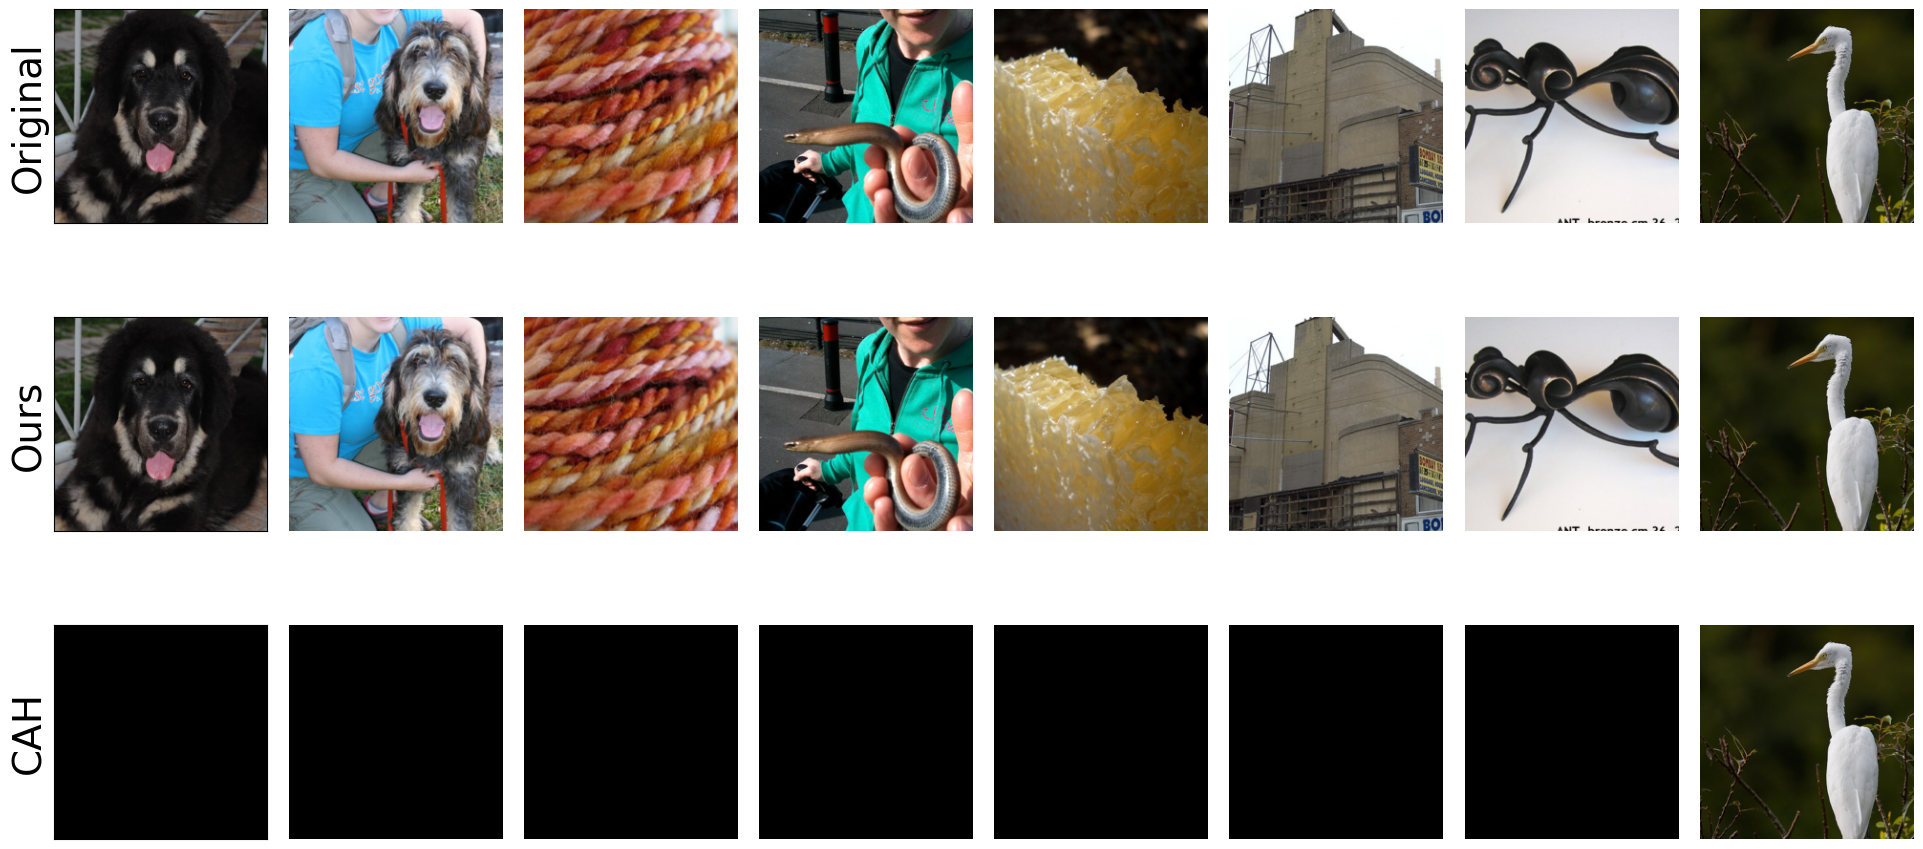
\includegraphics[scale=0.2]{assets/chapter_3/imagenet/reconstruct_img.png}
     \caption{The recovered images from a batch containing 1024 samples from ImageNet. The first row shows the original images, the second row the recovery of our attack after 10 rounds, and the last row shows that the baseline is not able to recover most of the images. } \label{fig:images_examples1}

\end{figure*}


We compare our method against the \emph{Curious Abandon Honesty} (CAH) attack~\cite{boenischWhenCuriousAbandon2023}. To provide a fair comparison with our iterative attack, we allow CAH to be executed across multiple communication rounds. Each experiment is repeated three times using different random seeds to assess the consistency of the results. Additional details on the configuration and parameter initialization of both attacks are provided in Appendix~\ref{app:model_init}.




\subsection{Experimental Results}\label{sec:exp_results}
\begin{figure*}[htbp]
    \centering
    \begin{subfigure}[b]{0.32\linewidth}
        \centering
        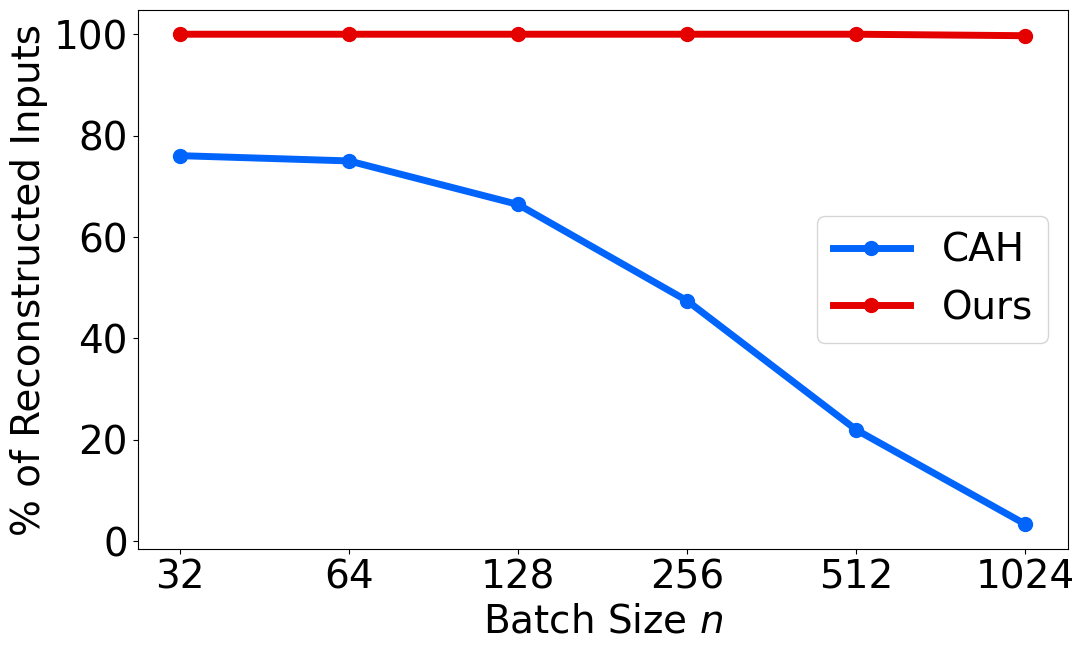
\includegraphics[width=\linewidth]{assets/chapter_3/imagenet/batch_size_effect.png}
        \caption{ImageNet}
        \label{fig:batch_eff_imagenet}
    \end{subfigure}\hfill
    \begin{subfigure}[b]{0.32\linewidth}
        \centering
        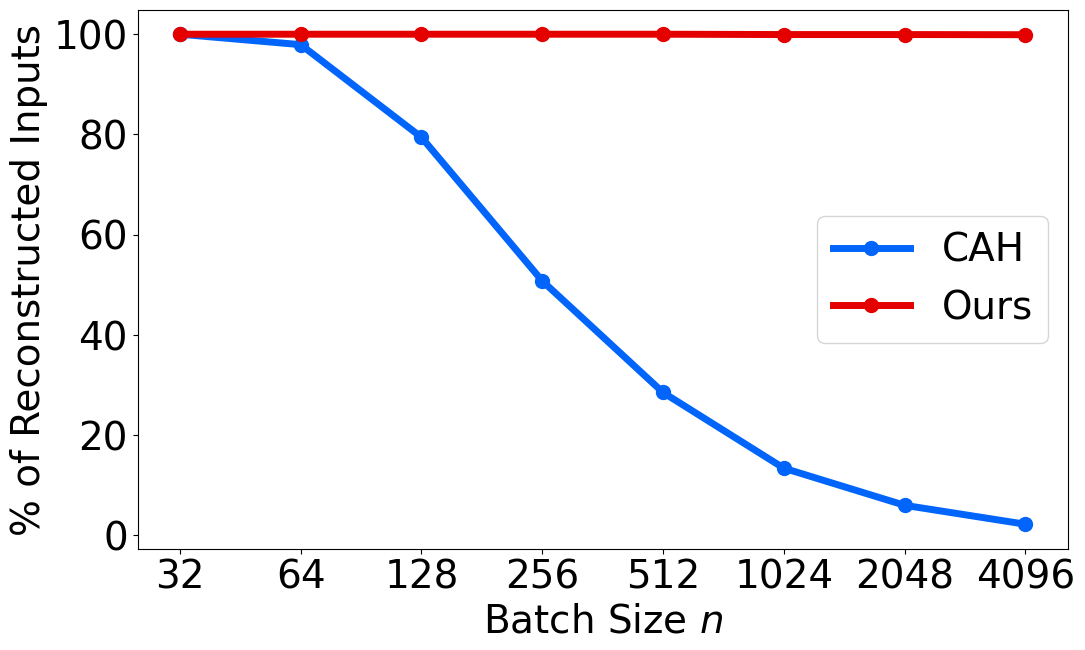
\includegraphics[width=\linewidth]{assets/chapter_3/harus/batch_size_effect.png}
        \caption{HARUS}
        \label{fig:batch_eff_harus}
    \end{subfigure}\hfill
    \begin{subfigure}[b]{0.32\linewidth}
        \centering
        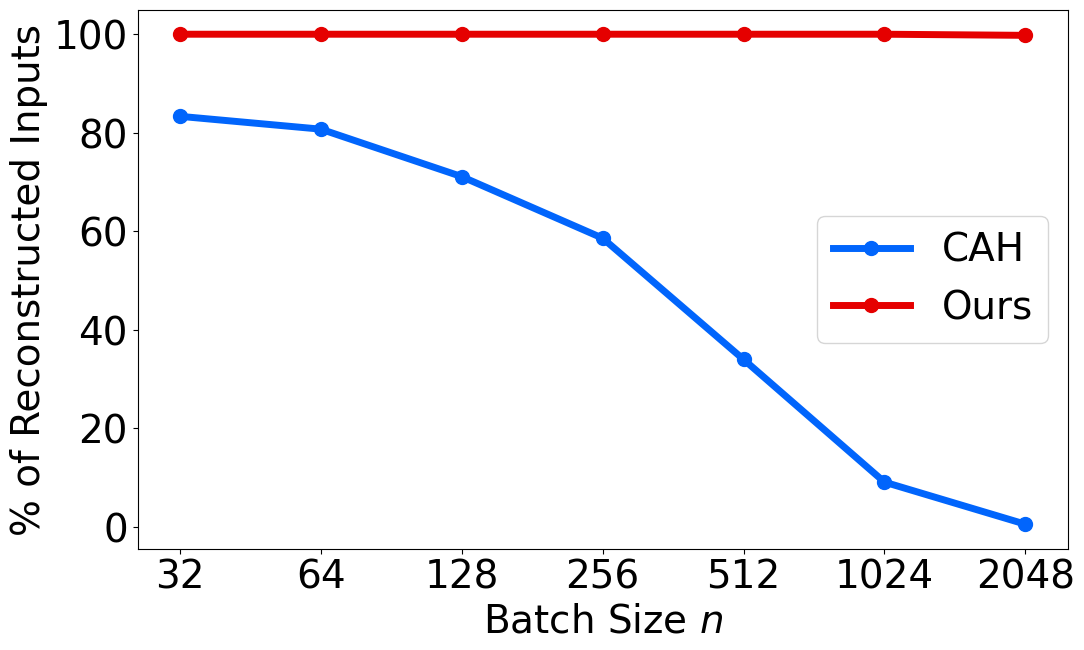
\includegraphics[width=\linewidth]{assets/chapter_3/cifar/batch_size_effect.png}
        \caption{CIFAR-10}
        \label{fig:batch_eff_cifar}
    \end{subfigure}
    \caption{Percentage of perfectly reconstructed inputs as a function of batch size on ImageNet, HARUS, and CIFAR-10, using a two-layer FC-NN with $N=1000$ neurons in the first layer. The number of communication rounds is fixed to $10$ for ImageNet, $50$ for HARUS, and $20$ for CIFAR-10.}
    \label{fig:batch_size_effect}
\end{figure*}
\subsubsection{Effect of Batch Size}
The experimental results show that our attack consistently outperforms CAH across all three datasets as the batch size increases. On ImageNet, after 10 communication rounds, our attack recovers the entire batch for every tested batch size, while maintaining a clear advantage over the baseline (Figure~\ref{fig:batch_eff_imagenet}). A similar behavior is observed on HARUS, where our attack successfully reconstructs batches of up to 4096 data points after 50 rounds (Figure~\ref{fig:batch_eff_harus}), and on CIFAR-10 (Figure~\ref{fig:batch_eff_cifar}), where it achieves complete reconstruction for batches of up to 2048 samples after 20 rounds.

In contrast, across all datasets, the fraction of samples reconstructed by CAH decreases as the batch size grows. This behavior highlights the limitations of sparsity-based attacks in recovering increasingly large batches when the input dimension is held constant, consistently with our theoretical findings presented in Section~\ref{sec:limit}.

\subsubsection{Effect of Communication Rounds}
\begin{figure*}[htbp]
    \centering
    \begin{subfigure}[b]{0.32\linewidth}
        \centering
        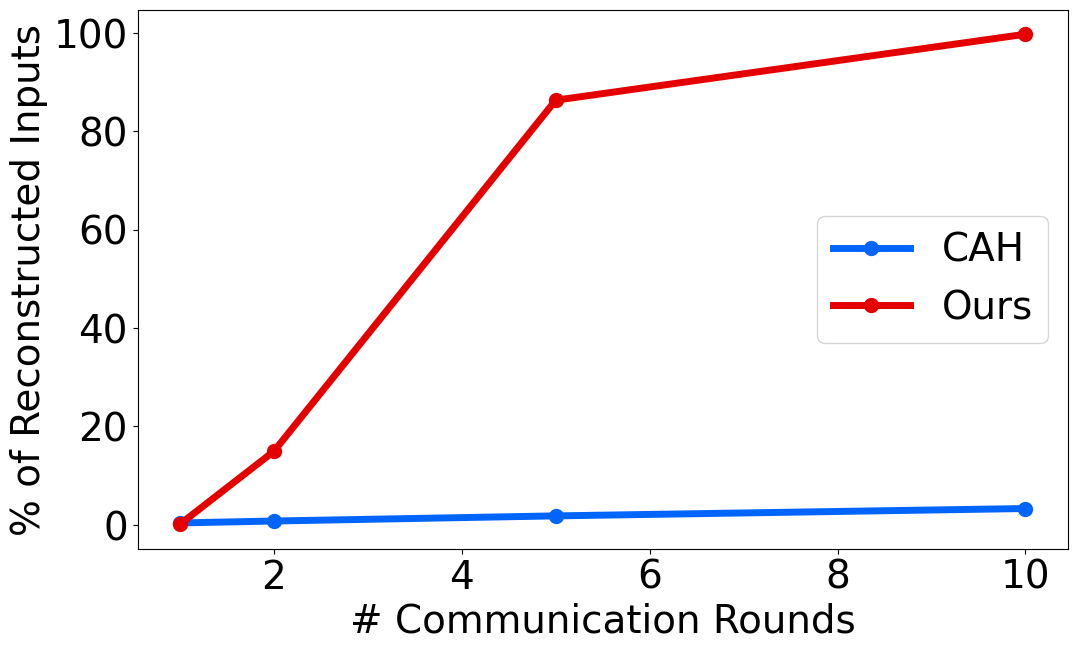
\includegraphics[height=0.60\linewidth]{assets/chapter_3/imagenet/rounds_effect.png}
        \caption{ImageNet}
        \label{fig:rounds_eff_imagenet}
    \end{subfigure}\hfill
    \begin{subfigure}[b]{0.32\linewidth}
        \centering
        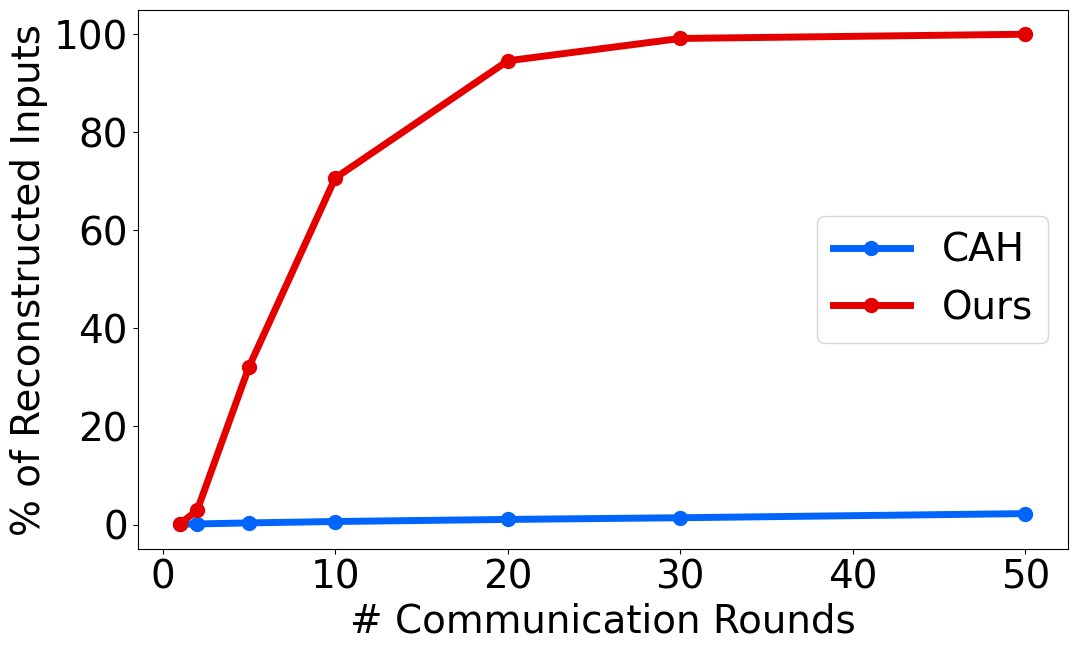
\includegraphics[height=0.60\linewidth]{assets/chapter_3/harus/rounds_effect.png}
        \caption{HARUS}
        \label{fig:rounds_eff_harus}
    \end{subfigure}\hfill
    \begin{subfigure}[b]{0.32\linewidth}
        \centering
        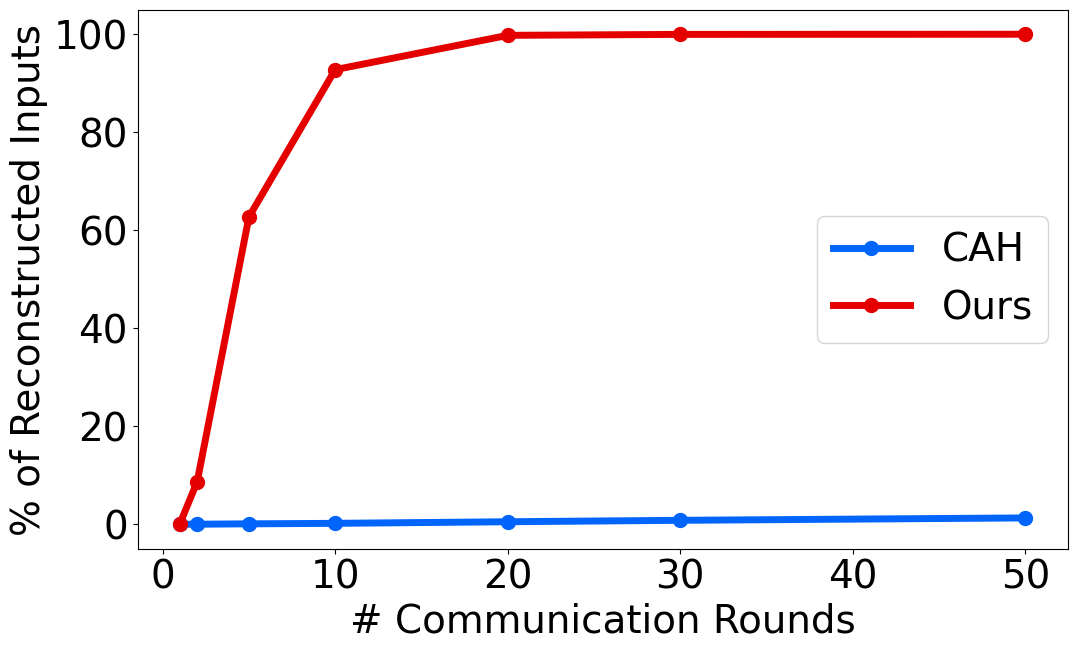
\includegraphics[height=0.60\linewidth]{assets/chapter_3/cifar/rounds_effect.png}
        \caption{CIFAR-10}
        \label{fig:rounds_eff_cifar}
    \end{subfigure}
    \caption{Percentage of perfectly reconstructed inputs as a function of the number of communication rounds on ImageNet, HARUS, and CIFAR-10, using a two-layer FC-NN with $N=1000$ neurons in the first layer. The batch size is fixed to $1,024$ for ImageNet, $4096$ for HARUS, and $2048$ for CIFAR-10.}
    \label{fig:batch_size_effect}
\end{figure*}

Figures~\ref{fig:rounds_eff_imagenet}, \ref{fig:rounds_eff_harus}, and~\ref{fig:rounds_eff_cifar} illustrate the effect of the communication budget on the reconstruction performance for large batches of $1,024$, $4096$, and $2048$ samples on ImageNet, HARUS, and CIFAR-10, respectively. After the first communication round, both attacks recover only a small fraction of the targeted batch. However, as additional rounds become available, the reconstruction rate of our method increases rapidly, eventually reaching complete reconstruction on all three datasets. This behavior reflects the iterative nature of our parallel search, where the information collected at each round identifies the regions that still contain unresolved samples and guides the placement of new hyperplanes in subsequent rounds.

In contrast, the baseline benefits only marginally from additional communication rounds. Repeating the attack allows it to explore new randomly sampled directions and potentially isolate additional samples, but its reconstruction remains restricted to inputs that can be separated from the rest of the batch by a single hyperplane. Consequently, additional rounds cannot overcome the geometric limitation characterized in Section~\ref{sec:limit}, whereas our attack can progressively isolate samples that cannot be recovered through a sparsity-based strategy.

\subsubsection{Reconstruction Performance Across Attack Regimes}

\begin{figure*}[htbp]
    \centering
    \begin{subfigure}[b]{0.32\linewidth}
        \centering
        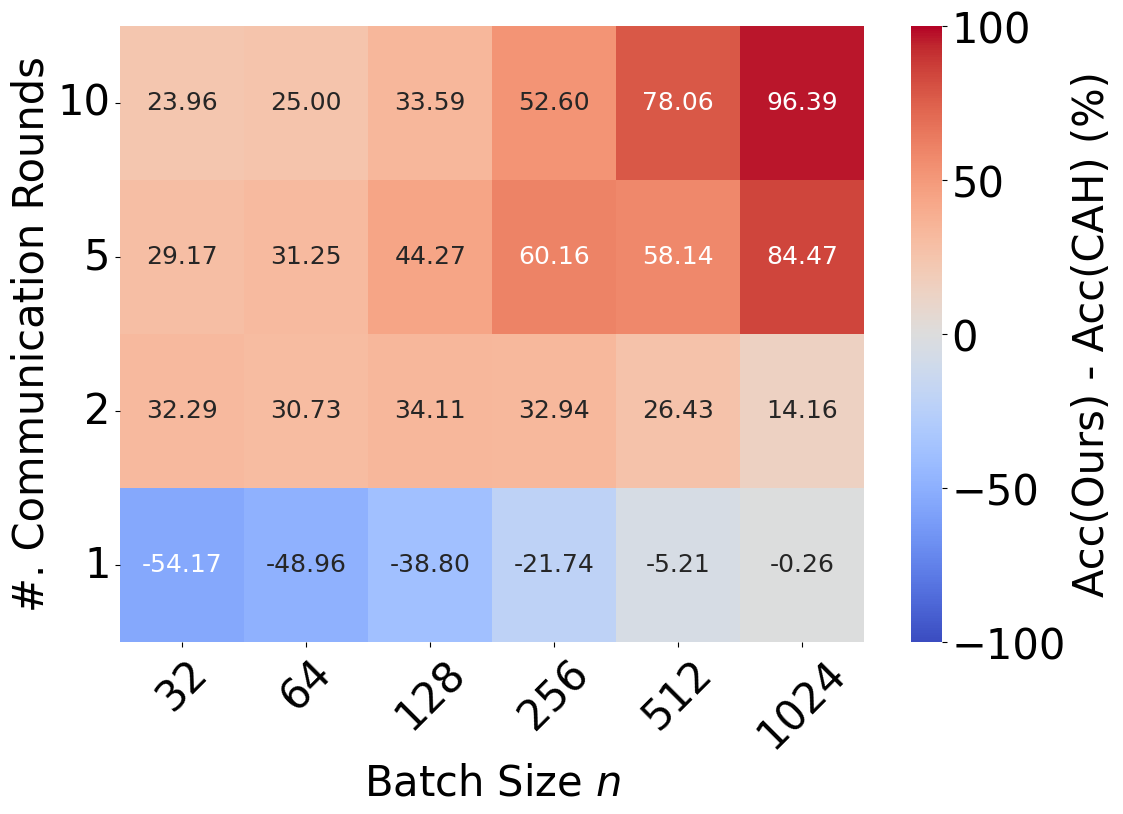
\includegraphics[height=0.64\linewidth]{assets/chapter_3/imagenet/heatmap.png}
        \caption{ImageNet}
        \label{fig:heatmap_imagenet}
    \end{subfigure}\hfill
    \begin{subfigure}[b]{0.32\linewidth}
        \centering
        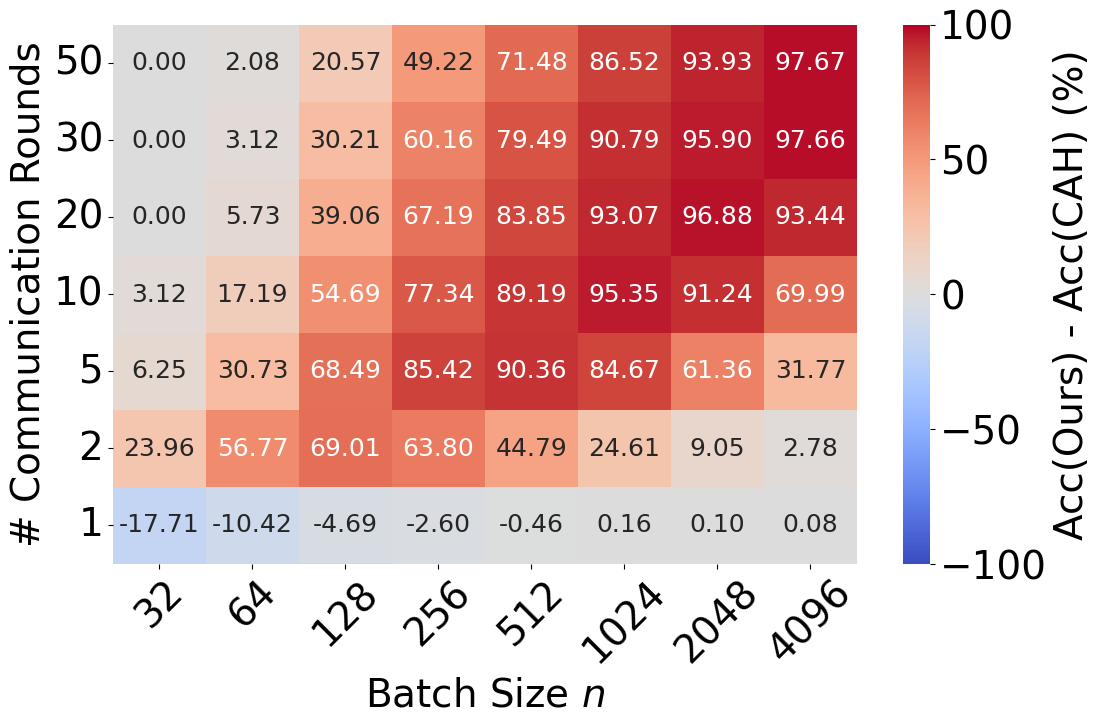
\includegraphics[height=0.64\linewidth]{assets/chapter_3/harus/heatmap.png}
        \caption{HARUS}
        \label{fig:heatmap_harus}
    \end{subfigure}\hfill
    \begin{subfigure}[b]{0.32\linewidth}
        \centering
        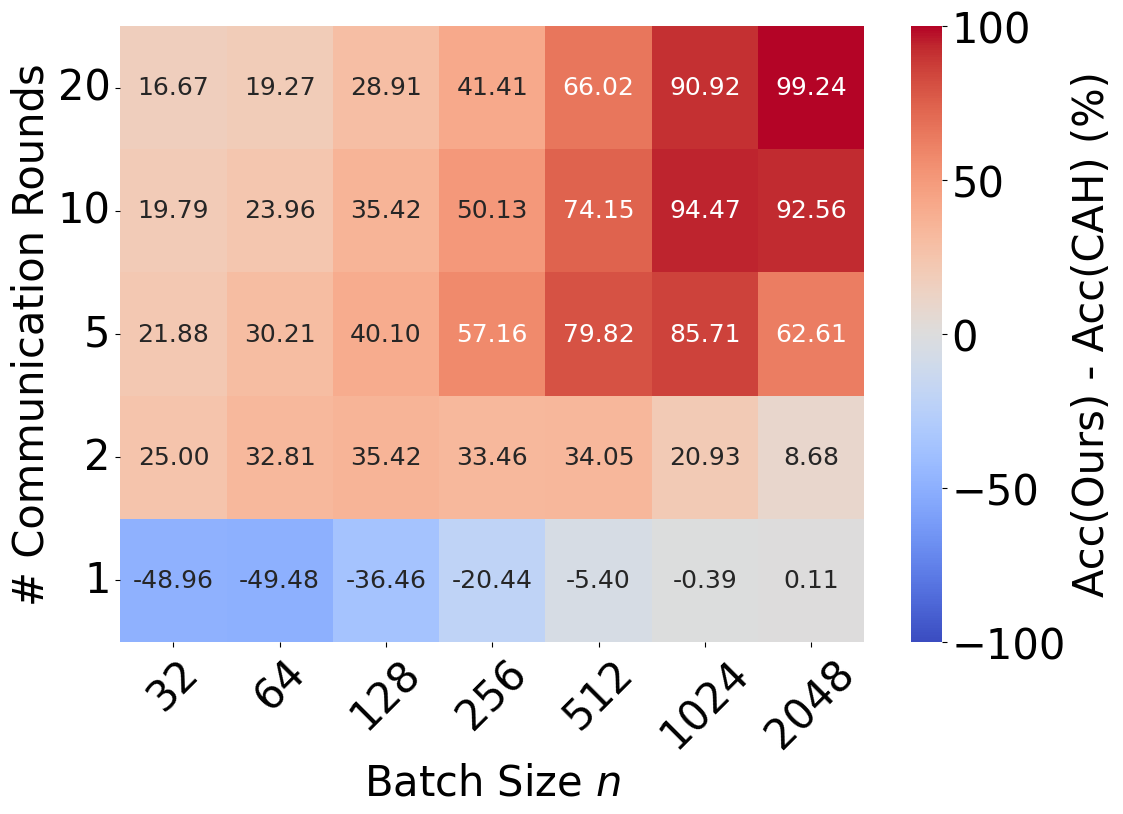
\includegraphics[height=0.64\linewidth]{assets/chapter_3/cifar/heatmap.png}
        \caption{CIFAR-10}
        \label{fig:heatmap_cifar}
    \end{subfigure}
    \caption{Percentage of perfectly reconstructed inputs as a function of the number of communication rounds on ImageNet, HARUS, and CIFAR-10, using a two-layer FC-NN with $N=1000$ neurons in the first layer. The batch size is fixed to $1,024$ for ImageNet, $4096$ for HARUS, and $2048$ for CIFAR-10.}
    \label{fig:heatmaps}
\end{figure*}

Figures~\ref{fig:heatmap_imagenet}, \ref{fig:heatmap_harus}, and~\ref{fig:heatmap_cifar} provide a more complete view of the relative performance of our attack and CAH across different batch sizes and communication budgets. Two key trends consistently emerge across the three datasets. First, the performance gap increasingly favors our attack as both the batch size and the number of communication rounds grow. The largest differences are therefore observed in the large-batch, multi-round regime, reaching $97.75$ percentage points on HARUS after 50 rounds for a batch of $4096$ samples and approximately $99$ percentage points on CIFAR-10 after 20 rounds for a batch of $2048$ samples. On ImageNet, our attack similarly outperforms CAH across all the evaluated multi-round settings.

Second, the different regions of the heatmaps highlight the regimes in which the two approaches are most effective. CAH can achieve better performance for small batches and, particularly on image data, during the first communication round. This initial advantage is relies on its ability to explore multiple random directions simultaneously, increasing the probability of immediately isolating some inputs. Moreover the trap weights initialization requires the attacker to have access to some representative data to tune some hyperparameters (see App.~\ref{app:model_init}), whereas our attack does not assume access to such auxiliary information (see Appendix~\ref{app:model_init}). These advantages are most beneficial in the small-batch and one-shot regimes, but rapidly diminish as the batch size grows. Conversely, the large-batch, multi-round region increasingly favors our attack, since additional communication rounds allow the geometric search to progressively refine the unexplored intervals and isolate samples that cannot be separated through the sparsity-based strategy of CAH. The consistent behavior across HARUS, CIFAR-10, and ImageNet therefore confirms that our approach is particularly effective in the large batches regime.

\subsubsection{Effect of the Number of Attack Neurons}

We also evaluate the effect of the number of neurons $N$ in the fully connected attack layer and its relationship with attack accuracy, see Table~\ref{tab:neuron_effect}.
While we observe that the percentage of reconstructed data increases with a larger number of neurons for both attacks, our attack outperforms the baseline in all but one combination of rounds and neuron counts. In many cases, our attack reconstructs nearly 100 times more inputs than CAH. We highlight a key distinction: the baseline reconstructs around 3.6\% of the input after 50 rounds with 2000 neurons, i.e., using 100 000 different random hyperplanes.
On the other hand, our attack manages to reconstruct 38\% of the batch after only 10 rounds with only 500 neurons, i.e., using only 5000 different hyperplanes.
In comparison, our attack reconstructs more than 10 times as many input points using 20 times fewer hyperplanes than the baseline,  thanks to its efficient search procedure for correctly positioning the hyperplanes that isolate the inputs.

\begin{table}[t]
    \centering
    \footnotesize
    \setlength{\tabcolsep}{3.5pt}
    \renewcommand{\arraystretch}{1.08}
    \caption{Effect of the number of neurons $N$ in the reconstruction layer. Values report the percentage of exactly reconstructed inputs on HARUS for $n=4096$ as mean $\pm$ standard deviation. The higher mean for each configuration is shown in bold.}
    \label{tab:neuron_effect}
    \begin{tabular}{@{}clcccccc@{}}
        \toprule
        \textbf{Rounds} & \textbf{Attack}
        & \multicolumn{6}{c}{\textbf{Number of neurons $N$}} \\
        \cmidrule(l){3-8}
        & & \textbf{100} & \textbf{200} & \textbf{500}
          & \textbf{1000} & \textbf{1500} & \textbf{2000} \\
        \midrule
        \multirow{2}{*}{1}
        & Ours & $0.00 \pm 0.00$ & $\mathbf{0.20} \pm 0.03$ & $\mathbf{0.05} \pm 0.02$
               & $\mathbf{0.15} \pm 0.06$ & $\mathbf{0.15} \pm 0.10$ & $\mathbf{0.21} \pm 0.09$ \\
        & CAH  & $\mathbf{0.01} \pm 0.03$ & $0.02 \pm 0.01$ & $0.04 \pm 0.01$
               & $0.07 \pm 0.04$ & $0.13 \pm 0.02$ & $0.15 \pm 0.05$ \\
        \midrule
        \multirow{2}{*}{5}
        & Ours & $\mathbf{1.11} \pm 0.31$ & $\mathbf{2.82} \pm 0.37$ & $\mathbf{9.33} \pm 4.66$
               & $\mathbf{31.93} \pm 1.80$ & $\mathbf{49.60} \pm 0.80$ & $\mathbf{64.80} \pm 2.08$ \\
        & CAH  & $0.07 \pm 0.03$ & $0.08 \pm 0.01$ & $0.20 \pm 0.04$
               & $0.33 \pm 0.06$ & $0.50 \pm 0.03$ & $0.66 \pm 0.09$ \\
        \midrule
        \multirow{2}{*}{10}
        & Ours & $\mathbf{3.11} \pm 0.88$ & $\mathbf{8.33} \pm 2.70$ & $\mathbf{38.02} \pm 1.54$
               & $\mathbf{70.87} \pm 1.44$ & $\mathbf{86.54} \pm 0.44$ & $\mathbf{93.17} \pm 0.19$ \\
        & CAH  & $0.08 \pm 0.06$ & $0.15 \pm 0.03$ & $0.31 \pm 0.07$
               & $0.62 \pm 0.01$ & $0.81 \pm 0.09$ & $1.06 \pm 0.08$ \\
        \midrule
        \multirow{2}{*}{30}
        & Ours & $\mathbf{21.10} \pm 1.44$ & $\mathbf{51.64} \pm 1.57$ & $\mathbf{88.38} \pm 0.58$
               & $\mathbf{99.06} \pm 0.29$ & $\mathbf{99.85} \pm 0.10$ & $\mathbf{99.98} \pm 0.03$ \\
        & CAH  & $0.25 \pm 0.07$ & $0.37 \pm 0.09$ & $0.78 \pm 0.09$
               & $1.38 \pm 0.08$ & $1.85 \pm 0.13$ & $2.46 \pm 0.20$ \\
        \midrule
        \multirow{2}{*}{50}
        & Ours & $\mathbf{42.52} \pm 2.07$ & $\mathbf{75.36} \pm 1.68$ & $\mathbf{97.84} \pm 0.21$
               & $\mathbf{99.98} \pm 0.03$ & $\mathbf{100.00} \pm 0.00$ & $\mathbf{100.00} \pm 0.00$ \\
        & CAH  & $0.37 \pm 0.07$ & $0.53 \pm 0.12$ & $1.24 \pm 0.24$
               & $2.23 \pm 0.10$ & $2.70 \pm 0.12$ & $3.62 \pm 0.47$ \\
        \bottomrule
    \end{tabular}
\end{table}

\subsubsection{Effect of Client Data Distribution}
We evaluate the performance of our attack under both IID and non-IID data distributions. Table~\ref{tab:effect_data_dist} reports results on the ImageNet dataset across different batch sizes and numbers of attack rounds.

In the IID setting, each client samples images uniformly at random from all 1,000 available classes. To simulate a non-IID scenario, we assign each client $i$ a distinct subset of classes $\mathcal{C}_i$ such that $\mathcal{C}_i\cap \mathcal{C}_j = \emptyset$, for any $i\not=j$. The result is that the local datasets of two clients do not share any common label. Each local dataset $\dataset_i$ is constructed by sequentially sampling 50 images per class from $\mathcal{C}_i$ until the desired dataset size is reached.
Our results indicate that the attack remains highly effective in both settings. In particular, the attacker successfully reconstructs the entire dataset within 10, and 20 attack rounds for batch sizes of 512, and 1024, respectively. While performance in the non-IID setting is occasionally slightly worse than in the IID case, this difference is marginal. One possible explanation lies in the spatial distribution of the data: the expected distance between two images randomly sampled from a subset of classes is smaller than the expected distance between two images sampled from the full set of classes. As a result, from a geometrical perspective, it becomes more challenging to position hyperplanes that isolate a single image, as $\Delta$ in \eqref{eq:final_rounds_bound} will be smaller than in the IID case.
\begin{table}[t]
    \centering
    \scriptsize
    \setlength{\tabcolsep}{2.5pt}
    \renewcommand{\arraystretch}{1.08}
    \caption{Effect of the client data distribution on ImageNet. Values report the percentage of exactly reconstructed inputs as mean $\pm$ standard deviation for different batch sizes and numbers of communication rounds. The higher mean for each configuration is shown in bold.}
    \label{tab:effect_data_dist}
    \begin{tabular}{@{}clcccccc@{}}
        \toprule
        \textbf{Rounds} & \textbf{Distribution}
        & \multicolumn{6}{c}{\textbf{Batch size}} \\
        \cmidrule(l){3-8}
        & & \textbf{32} & \textbf{64} & \textbf{128}
          & \textbf{256} & \textbf{512} & \textbf{1024} \\
        \midrule
        \multirow{2}{*}{2}
        & Non-IID & $95.83 \pm 3.61$ & $\mathbf{88.54} \pm 1.80$ & $\mathbf{77.60} \pm 3.93$
                  & $62.11 \pm 5.12$ & $38.87 \pm 2.71$ & $\mathbf{17.68} \pm 0.29$ \\
        & IID     & $\mathbf{100.00} \pm 0.00$ & $88.02 \pm 0.90$ & $74.74 \pm 7.86$
                  & $\mathbf{62.63} \pm 7.25$ & $\mathbf{39.00} \pm 4.48$ & $\mathbf{17.68} \pm 0.93$ \\
        \midrule
        \multirow{2}{*}{5}
        & Non-IID & $\mathbf{100.00} \pm 0.00$ & $\mathbf{100.00} \pm 0.00$ & $99.48 \pm 0.90$
                  & $99.22 \pm 0.78$ & $96.55 \pm 0.49$ & $86.23 \pm 1.61$ \\
        & IID     & $\mathbf{100.00} \pm 0.00$ & $\mathbf{100.00} \pm 0.00$ & $\mathbf{100.00} \pm 0.00$
                  & $\mathbf{99.74} \pm 0.45$ & $\mathbf{97.92} \pm 1.13$ & $\mathbf{87.14} \pm 0.91$ \\
        \midrule
        \multirow{2}{*}{10}
        & Non-IID & $\mathbf{100.00} \pm 0.00$ & $\mathbf{100.00} \pm 0.00$ & $\mathbf{100.00} \pm 0.00$
                  & $\mathbf{100.00} \pm 0.00$ & $\mathbf{100.00} \pm 0.00$ & $99.35 \pm 0.41$ \\
        & IID     & $\mathbf{100.00} \pm 0.00$ & $\mathbf{100.00} \pm 0.00$ & $\mathbf{100.00} \pm 0.00$
                  & $\mathbf{100.00} \pm 0.00$ & $\mathbf{100.00} \pm 0.00$ & $\mathbf{99.61} \pm 0.34$ \\
        \midrule
        \multirow{2}{*}{20}
        & Non-IID & $\mathbf{100.00} \pm 0.00$ & $\mathbf{100.00} \pm 0.00$ & $\mathbf{100.00} \pm 0.00$
                  & $\mathbf{100.00} \pm 0.00$ & $\mathbf{100.00} \pm 0.00$ & $\mathbf{100.00} \pm 0.00$ \\
        & IID     & $\mathbf{100.00} \pm 0.00$ & $\mathbf{100.00} \pm 0.00$ & $\mathbf{100.00} \pm 0.00$
                  & $\mathbf{100.00} \pm 0.00$ & $\mathbf{100.00} \pm 0.00$ & $\mathbf{100.00} \pm 0.00$ \\
        \bottomrule
    \end{tabular}
\end{table}

\subsubsection{Effect of Multiple Local Steps}\label{sec:local_steps_effect}

We next relax the full-batch FedSGD assumption and consider a setting in which the client performs $K>1$ local gradient steps before returning its update to the server. As discussed later in Section~\ref{sec:conclusions}, this setting makes reconstruction more challenging because both $\Win$ and $\bin$ are updated during local training. Consequently, the directions and positions of the hyperplanes change across local steps, preventing the attacker from maintaining the precise geometric partition used in the full-batch setting.

To mitigate this effect, we adapt the malicious model so that the updates of the attacked layer remain small relative to the magnitude of its parameters. In particular, we aim to keep the gradients $\frac{\partial \loss}{\partial \Win}$ and $\frac{\partial \loss}{\partial \bin}$ sufficiently small so that the corresponding hyperplanes move only slightly during local training. Since observations obtained after multiple local steps are no longer expected to coincide exactly, we also replace the exact comparison used in the original attack with an approximate criterion. The complete parameter initialization and implementation details are provided in Appendix~\ref{par:local_steps}.

We evaluate this extension on CIFAR-10 by considering one local epoch divided into multiple minibatch updates. The targeted client holds $|\dataset|=1024$ images, where $|\dataset|$ denotes the size of the client's local dataset and is distinct from the minibatch size $n$. We vary the minibatch size as $n\in\{2^3,2^4,\ldots,2^{10}\}$, resulting in $K=|\dataset|/n$ local steps, and use a learning rate of $10^{-4}$.

Figure~\ref{fig:minibatch} shows that reconstruction becomes progressively more difficult as the number of local steps increases. Nevertheless, our attack remains effective in the multi-step setting, recovering up to approximately $35\%$ of the client's images, whereas CAH remains below $20\%$ under the same experimental conditions. We also consider a more demanding setting than the original evaluation of CAH~\cite{boenischWhenCuriousAbandon2023}, which uses $K=5$ local steps and a local dataset of $|\dataset|=200$ samples. These results provide preliminary evidence that the attack can tolerate multiple minibatch updates within one local epoch, although extending it to cumulative updates over multiple local epochs remains an open problem.

\begin{figure}[t]
    \centering
    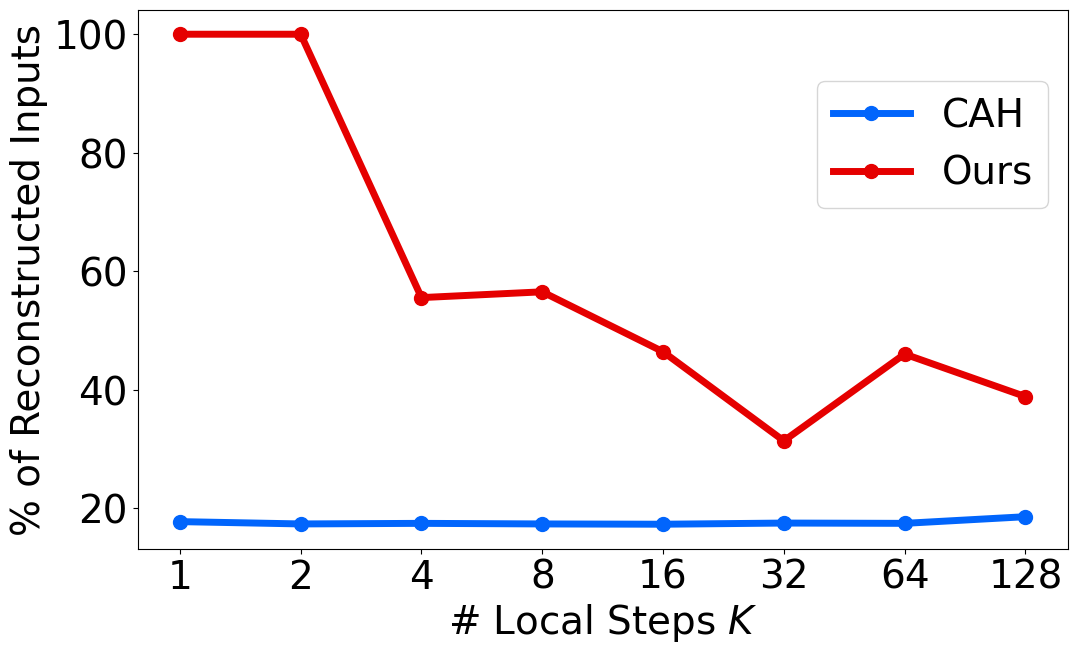
\includegraphics[width=0.6\linewidth]{assets/chapter_3/cifar/minibatch_effect.png}
    \caption{Percentage of perfectly reconstructed CIFAR-10 inputs as a function of the number of local steps $K$. The client dataset contains $1024$ images, and the training batch size is $n=1024/K$. The reconstruction is evaluated after $50$ communication rounds.}
    \label{fig:minibatch}
\end{figure}

\francesco{verifica di nuovo questi risultati e se mantenerli nella tesi}

\subsubsection{Effect of Noise}\label{sec:exp_noise}

To assess the robustness of our attack, we conduct experiments in the presence of noise, which may arise from imperfections in real-world communication channels or from defense mechanisms implemented by the client to defend against privacy attacks, Adding noise directly affects the gradient observations used by our attack and therefore interferes with both the localization and reconstruction of individual samples.

To improve robustness in this setting, the malicious server can adapt the model parameters to increase the magnitude of the gradients carrying information about the client inputs. This improves the signal-to-noise ratio of the observations available to the attacker and reduces the relative influence of the perturbation. Interestingly, this modification follows the opposite principle from the one used in the multiple-local-step setting: there, the objective is to keep the attacked-layer gradients small in order to preserve the hyperplane positions during local training, whereas here the objective is to amplify them so that the data-dependent signal remains distinguishable from the added noise. The corresponding parameter initialization is detailed in Appendix~\ref{app:noise}.

Figure~\ref{fig:noise_effect} reports the reconstruction performance for different communication budgets and levels of Gaussian noise. The targeted client holds $1024$ CIFAR-10 images and computes a full-batch FedSGD update using a learning rate of $10^{-4}$. As expected, increasing the noise level reduces the fraction of perfectly reconstructed samples. Nevertheless, our attack remains substantially more effective than CAH across the evaluated noise levels. While the reconstruction rate of our method decreases progressively as stronger noise is introduced, CAH does not recover any sample for either of the considered non-zero noise levels, with the corresponding curves overlapping in Figure~\ref{fig:noise_effect}. As a result, our method retains a reconstruction advantage of almost $40$ percentage points in the tested noisy settings.



\begin{figure}[h]
    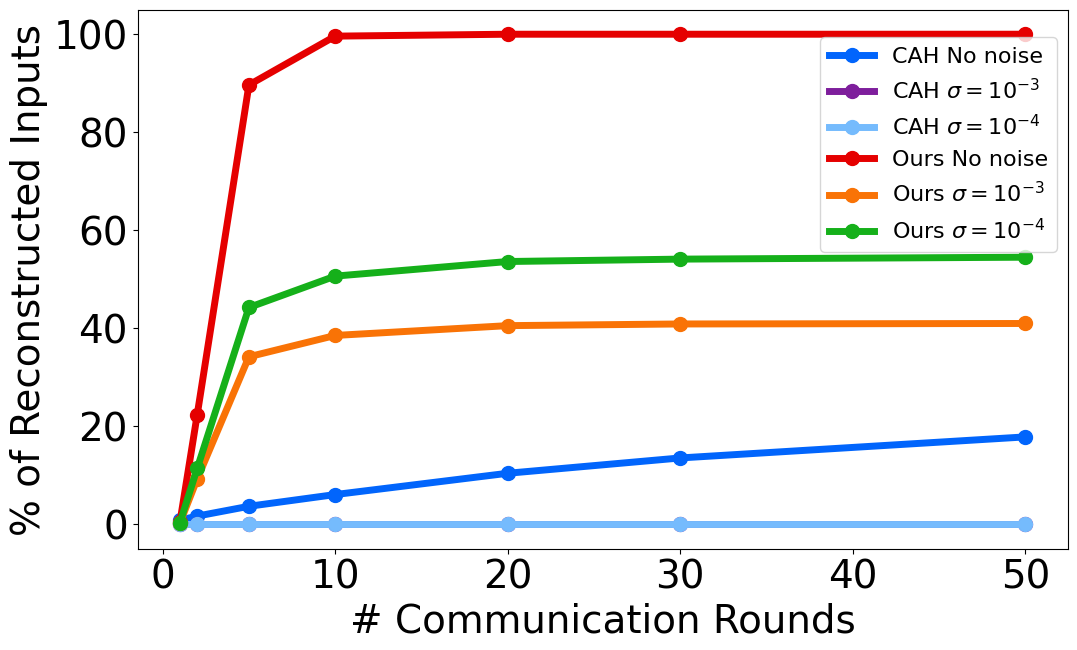
\includegraphics[width=0.7\linewidth]{assets/chapter_3/cifar/dp_effect.png}
    \centering
    \caption{Percentage of perfectly reconstructed CIFAR-10 inputs as a function of the number of communication rounds under different levels of Gaussian noise variance $\sigma$. The targeted client holds $1024$ images and trains a two-layer FC-NN with $N=1000$ neurons in the first layer using full-batch FedSGD.}
    \label{fig:noise_effect}
\end{figure}



\subsubsection{Effect of the Number of Hidden Layers}

As discussed in Section~\ref{sec:our_attack}, our method can be easily adapted to any fully-connected neural network with $L$ layers with ReLU activation function. The extension is described in details in Appendix~\ref{app:gener_nn}. Here, we present the results on ImageNet using models with 1, 2, 3, and 4 hidden layers. The first layer has  $N=1000$, while each subsequent layer consists of 100 neurons.  We set the malicious parameters of the input and classification layers as described in App.~\ref{app:model_init}, and generate the columns of each additional hidden layer from $\mathcal{N}(0, 10^{-6})$. The corresponding bias terms are also scaled by a $10^{-3}$ factor. Table~\ref{tab:layers_effect} demonstrates that, regardless of the number of hidden layers, the reconstruction accuracy of the attack exhibits only minor fluctuations caused by numerical precision, confirming that the number of layers does not significantly affect the performance of our attack.

\begin{table}[t]
    \centering
    \setlength{\tabcolsep}{8pt}
    \renewcommand{\arraystretch}{1.08}
    \caption{Effect of the number of hidden layers. Values report the percentage of exactly reconstructed inputs on ImageNet for $n=512$ as mean $\pm$ standard deviation. The highest mean in each row is shown in bold.}
    \label{tab:layers_effect}
    \begin{tabular}{@{}ccccc@{}}
        \toprule
        \textbf{Rounds} & \multicolumn{4}{c}{\textbf{Number of hidden layers}} \\
        \cmidrule(l){2-5}
        & \textbf{1} & \textbf{2} & \textbf{3} & \textbf{4} \\
        \midrule
        1  & $\mathbf{0.20} \pm 0.00$ & $\mathbf{0.20} \pm 0.00$
           & $\mathbf{0.20} \pm 0.00$ & $\mathbf{0.20} \pm 0.00$ \\
        2  & $\mathbf{35.61} \pm 3.12$ & $35.16 \pm 3.32$
           & $35.29 \pm 3.33$ & $35.29 \pm 3.33$ \\
        3  & $\mathbf{78.38} \pm 2.79$ & $77.99 \pm 2.93$
           & $78.26 \pm 2.66$ & $78.19 \pm 2.74$ \\
        5  & $\mathbf{97.14} \pm 0.98$ & $97.01 \pm 1.19$
           & $\mathbf{97.14} \pm 0.98$ & $\mathbf{97.14} \pm 0.98$ \\
        7  & $\mathbf{99.74} \pm 0.45$ & $\mathbf{99.74} \pm 0.45$
           & $\mathbf{99.74} \pm 0.45$ & $\mathbf{99.74} \pm 0.45$ \\
        10 & $\mathbf{100.00} \pm 0.00$ & $\mathbf{100.00} \pm 0.00$
           & $\mathbf{100.00} \pm 0.00$ & $\mathbf{100.00} \pm 0.00$ \\
        \bottomrule
    \end{tabular}
\end{table}

\subsubsection{Attack on a Convolutional Neural Network}

To evaluate whether our attack extends beyond fully connected architectures, we consider a VGG-style convolutional neural network composed of three convolutional layers followed by two fully connected layers, following the architecture described in~\cite[Table~9]{boenischWhenCuriousAbandon2023}. As shown in Table~\ref{tab:cnn_effect}, our attack remains effective across all tested batch sizes and progressively improves as additional communication rounds become available. After 10 rounds, it reconstructs virtually the entire batch even for $n=1024$, reaching $99.54\%$ reconstruction accuracy, and after 20 rounds it achieves complete reconstruction for every evaluated batch size. In contrast, CAH degrades substantially as the batch size increases and recovers only $15.40\%$ of the samples for $n=1024$ after 20 rounds. These results show that the proposed attack can be successfully extended to convolutional architectures while preserving the scalability observed in the fully connected setting.

\begin{table}[t]
    \centering
    \footnotesize
    \setlength{\tabcolsep}{2pt}
    \renewcommand{\arraystretch}{1.08}
    \caption{Reconstruction performance on the VGG-style convolutional neural network. Values report the percentage of exactly reconstructed inputs as mean $\pm$ standard deviation for different batch sizes and numbers of communication rounds. The higher mean for each configuration is shown in bold.}
    \label{tab:cnn_effect}
    \begin{tabular}{@{}clcccccc@{}}
        \toprule
        \textbf{Rounds} & \textbf{Attack}
        & \multicolumn{6}{c}{\textbf{Batch size}} \\
        \cmidrule(l){3-8}
        & & \textbf{32} & \textbf{64} & \textbf{128}
          & \textbf{256} & \textbf{512} & \textbf{1024} \\
        \midrule
        \multirow{2}{*}{1}
        & Ours & $23.96 \pm 7.86$ & $12.50 \pm 4.13$ & $4.95 \pm 0.90$
               & $1.56 \pm 0.68$ & $0.72 \pm 0.30$ & $0.46 \pm 0.15$ \\
        & CAH  & $\mathbf{76.04} \pm 4.77$ & $\mathbf{65.62} \pm 2.71$ & $\mathbf{47.92} \pm 2.74$
               & $\mathbf{30.73} \pm 2.15$ & $\mathbf{11.59} \pm 1.08$ & $\mathbf{1.56} \pm 0.39$ \\
        \midrule
        \multirow{2}{*}{2}
        & Ours & $\mathbf{96.88} \pm 3.12$ & $\mathbf{95.31} \pm 2.71$ & $\mathbf{88.02} \pm 3.16$
               & $\mathbf{70.96} \pm 2.15$ & $\mathbf{53.91} \pm 2.73$ & $\mathbf{25.81} \pm 1.42$ \\
        & CAH  & $79.17 \pm 1.80$ & $71.88 \pm 4.13$ & $57.55 \pm 1.19$
               & $41.15 \pm 2.66$ & $18.68 \pm 2.07$ & $2.86 \pm 0.56$ \\
        \midrule
        \multirow{2}{*}{5}
        & Ours & $\mathbf{100.00} \pm 0.00$ & $\mathbf{100.00} \pm 0.00$ & $\mathbf{100.00} \pm 0.00$
               & $\mathbf{100.00} \pm 0.00$ & $\mathbf{99.15} \pm 0.41$ & $\mathbf{89.91} \pm 2.15$ \\
        & CAH  & $85.42 \pm 3.61$ & $78.12 \pm 5.41$ & $69.01 \pm 3.16$
               & $54.30 \pm 3.96$ & $27.86 \pm 1.30$ & $5.86 \pm 0.74$ \\
        \midrule
        \multirow{2}{*}{10}
        & Ours & $\mathbf{100.00} \pm 0.00$ & $\mathbf{100.00} \pm 0.00$ & $\mathbf{100.00} \pm 0.00$
               & $\mathbf{100.00} \pm 0.00$ & $\mathbf{100.00} \pm 0.00$ & $\mathbf{99.54} \pm 0.23$ \\
        & CAH  & $87.50 \pm 3.12$ & $84.38 \pm 0.00$ & $75.78 \pm 0.78$
               & $62.63 \pm 3.83$ & $38.74 \pm 0.74$ & $10.19 \pm 0.62$ \\
        \midrule
        \multirow{2}{*}{20}
        & Ours & $\mathbf{100.00} \pm 0.00$ & $\mathbf{100.00} \pm 0.00$ & $\mathbf{100.00} \pm 0.00$
               & $\mathbf{100.00} \pm 0.00$ & $\mathbf{100.00} \pm 0.00$ & $\mathbf{100.00} \pm 0.00$ \\
        & CAH  & $88.54 \pm 3.61$ & $88.54 \pm 2.39$ & $80.21 \pm 0.45$
               & $70.83 \pm 2.51$ & $48.83 \pm 0.59$ & $15.40 \pm 0.63$ \\
        \bottomrule
    \end{tabular}
\end{table}


 \subsubsection{Attack Runtime and Overhead}

In terms of computational overhead, we evaluate our attack on the most computationally demanding setting—ImageNet with $n=1024$. In this case, the attack requires less than two seconds per round (primarily for lines 9 and 11 in Alg.~\ref{algo:parallelattack}) and under four seconds for the final image reconstruction phase (line 12), using an NVIDIA GeForce RTX 2080 Ti GPU. Since attacks are carried out across consecutive rounds, this additional overhead of approximately two seconds per round is negligible compared to the tens of seconds typically required to transmit the model in a single communication round.


\section{Discussion}\label{sec}

Secure aggregation~\cite{secure_aggregation_bonawitz} is commonly proposed to protect individual client updates by allowing the server to observe only their aggregate. However, it does not eliminate the information exploited by our attack: from the attacker's perspective, aggregating the updates of multiple clients increases the number of data points contributing to the observed gradient. Since our method is designed to progressively isolate samples from large aggregated batches, a sufficiently large communication budget may still allow the server to reconstruct the underlying inputs. In this case, however, the reconstructed samples cannot necessarily be associated with the client from which they originated.

A more direct countermeasure against a malicious server is to perturb the information before it leaves the client, for example through local differential privacy (LDP)~\cite{dp_dwork}. Noise added locally modifies the gradient observations on which the attack relies, hindering both the localization and the exact reconstruction of individual samples. The experiments in Section~\ref{sec:ctp_experiments} confirm this effect: increasing the magnitude of Gaussian perturbations progressively reduces the fraction of perfectly reconstructed inputs. At the same time, they show that noise addition does not immediately prevent reconstruction, since the malicious server can adapt the model parameters to increase the magnitude of the data-dependent gradient signal. 

Our experimental evaluation shows that the attack is not limited to the simplified architectural and data assumptions used in its derivation. In particular, increasing the number of fully connected layers has only a negligible impact on reconstruction performance, and the attack can also be extended to convolutional architectures through existing model modifications. Moreover, the results remain unaffected by the client data distribution, with comparable reconstruction performance under both IID and non-IID settings. These experiments indicate that the geometric reconstruction strategy is robust to changes in both the model architecture and the distribution of the targeted data.

We also provide a preliminary evaluation beyond the full-batch FedSGD setting by considering one local epoch composed of multiple minibatch updates. In this case, the parameters of the attacked layer evolve during local training, causing the directions and positions of the malicious hyperplanes to change across local steps and making reconstruction more challenging. Despite this additional difficulty, our attack remains effective and consistently outperforms CAH across the evaluated configurations, recovering a substantially larger fraction of the targeted data. These results suggest that the proposed reconstruction strategy can tolerate a certain degree of local optimization, although performance progressively degrades as the number of local steps increases.



\section{Future Works and Conclusion}\label{sec:conclusions}

In this chapter, we introduced a novel analytical data reconstruction attack for federated classification tasks under a malicious-server threat model. By interpreting the activation boundaries of fully connected ReLU neurons geometrically, we first showed that existing sparsity-based attacks are fundamentally limited by their need to separate a sample from all other points in the batch. We then developed a different strategy in which parallel hyperplanes progressively partition the input space and isolate individual records across communication rounds. Given a sufficient communication budget, our \emph{Cutting Through Privacy} attack recovers the complete client dataset, overcoming the degradation of existing analytical attacks as the batch size grows.

The results presented in this chapter also motivate several directions for extending the attack beyond the setting considered in its original formulation. One important question concerns the interaction with stronger client-side privacy mechanisms. Our experiments in Section~\ref{sec:exp_results} show that Gaussian perturbations alone reduce reconstruction performance but do not necessarily prevent leakage against an adaptive malicious server. A natural next step is therefore to evaluate CTP against complete differential privacy mechanisms, in which gradient clipping and calibrated noise are jointly employed to satisfy a prescribed privacy budget. Such an analysis would provide a more systematic characterization of the privacy-utility trade-off required to prevent reconstruction.

Another open question concerns more general local training procedures. Our preliminary experiments already depart from full-batch FedSGD by considering several minibatch updates within a single local epoch, showing that reconstruction remains possible despite the resulting displacement of the malicious hyperplanes. Extending the attack to multiple local epochs would require tracking or compensating for this progressive evolution throughout the entire local optimization trajectory, and constitutes an important step toward more general federated optimization settings.

Finally, the attack could be extended to broader architectures and tasks. When the first fully connected layer operates on an intermediate representation, CTP can be combined with existing model inversion methods~\cite{kariyappaCocktailPartyAttack2023, ZHANG2023119421} to recover the original input. However, this second inversion step generally loses the exact-reconstruction property. Developing analytical end-to-end reconstruction methods for more complex architectures, as well as extending the gradient-control mechanism beyond classification, remains an important direction for future work.



